\chapter{\leavevmode\newline The Large Hadron Collider}
\label{chap:chapter_2}

The Large Hadron Collider (LHC) is the largest particle collider in the world. It is located inside a 26.7 km long underground tunnel in the facilities of the European Organization for Nuclear Research (CERN), near Ginebra. This tunnel was used in the past for the Large Positron-Electron Collider (LEP) before it was shut down in 2000.

The initial goal of the LHC was to detect the Higgs Boson. For this purpose, it began operations in 2008, but due to a malfunction incident, it was shut down until the end of 2009. Finally, the Higgs boson was detected in 2012. On top of that, many other predictions of the SM have been confirmed using the LHC experimental infrastructure, and it has also been possible to study the phenomena the SM cannot explain, as described in the previous chapter.

The LHC is able to produce proton-proton (p+p) collisions at energies up to 7 TeV and lead ions (Pb-Pb) collisions at 2.76 TeV. p-Pb collisions are also possible at 5.02 TeV \cite{vovchenko2019canonical} and are of special interest in this manuscript. For such collisions, two beams of the target particles are generated using the Proton Synchrotron (PS) and the Super Proton Synchrotron (SPS) and then accelerated in opposite directions at energies up to 460 GeV.

There are four points where collisions occur, and there is a detector associated with each point, as shown in fig \ref{fig:LHC}. Two of these detectors are for general purposes: A Toroidal LHC Apparatus (ATLAS) and Compact Muon Solenoid (CMS). The other two are the LHC beauty detector (LHCb) used to study heavy-flavor physics and indirect CP violations in b-mesons, and A Large Ion Collider Experiment (ALICE) used for heavy-ion collisions.

The results and analysis presented in later chapters are based on CMS. Therefore, a detailed description of this detector will be given in the next section.

\begin{figure}[htp!]
	\centering
	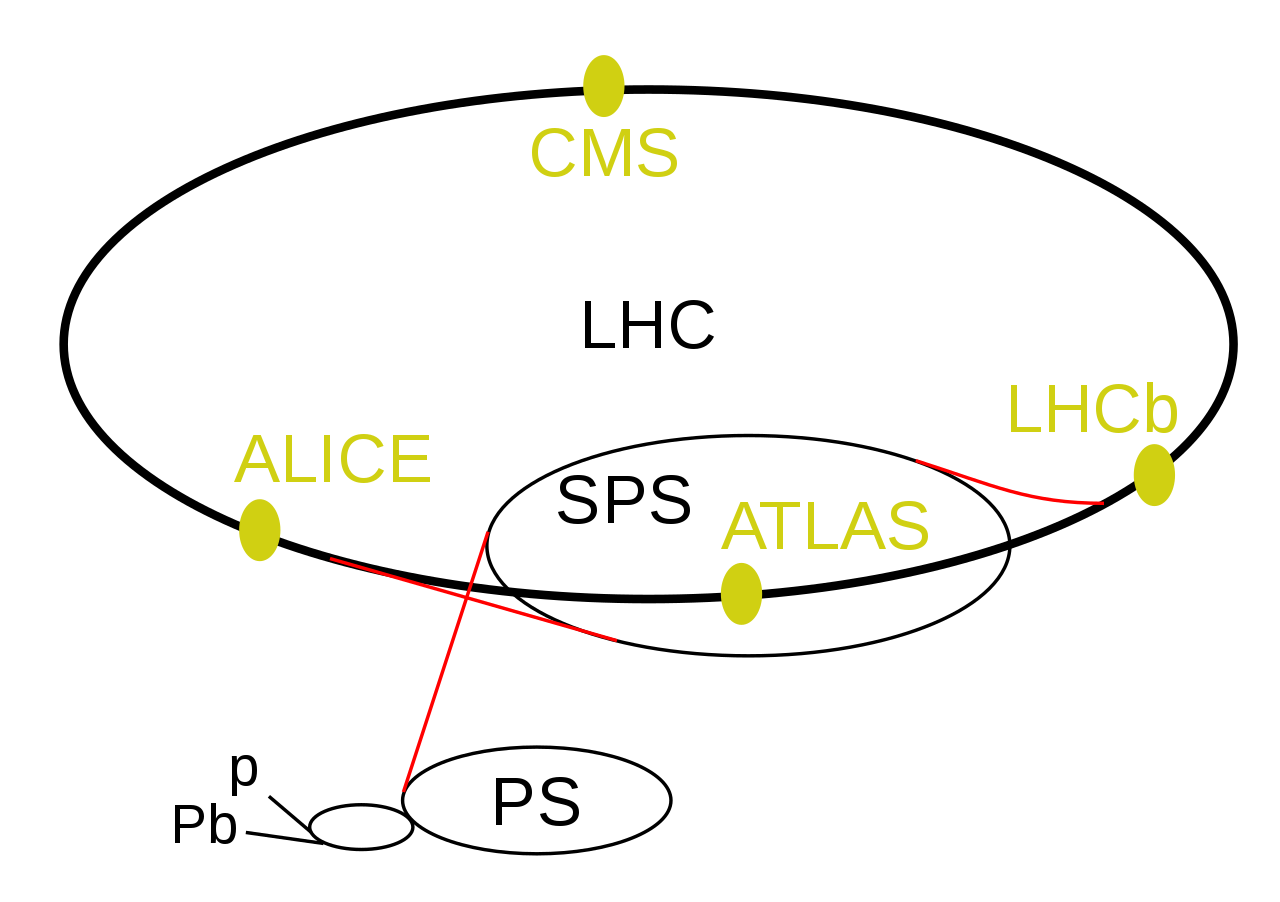
\includegraphics[scale=0.3]{MainContent/Figs/LHC.png}
	\caption{LHC experimental chain. The yellow dots represent the four main experiments. This figure was retrieved from }
	\label{fig:LHC}
\end{figure}

\section{The CMS Detector}

CMS is a general purpose detector used to reconstruct the decay products in proton and heavy-ion collisions at high energies. It can detect nearly any particle, specially muons, with high precision. CMS is located in a cavern about 100 m underground near Cessy, France. It has a cylindrical geometry, with a full length of 21.5 m and a diameter of 15 m. With a total weight of 12500 t, it is the heaviest detector in the LHC. CMS is operated by a large collaboration of members worldwide, consisting of over 4000 particle physicists, engineers, computer scientists, technicians, and students from around 200 institutes and universities from more than 40 countries \cite{cms_collab}.

The main feature of CMS is a superconducting solenoid able to produce a internal, uniform 4T magnetic field. Inside the solenoid, there is a tracking system  Before explaining with more detail the internal parts of the detector, the coordinate system will be introduced in the next subsection. 

\subsection{CMS coordinate system}
Called the rapidity and pseudorapidity.